\chapter{Introducción}

La clasificación de tráfico en red es una tarea importante 
en lo relativo a las comunicaciones, en un mundo cada vez 
más digitalizado e intercomunicado, lo que más importa es 
la seguridad y para ello es esencial la clasificación del 
tráfico, permitiendo detectar de forma temprana intrusiones 
y comportamientos anómalos, por ejemplo podríamos ver, mediante 
la clasificación del tráfico si estamos siendo atacados mediante 
denegación de servicio, \textit{DDoS}, y podríamos tomar medidas para cortar esa 
conexión. De esta forma, por ejemplo, el encargado de un 
servidor podrá mantener la calidad de servicio, pues mediante 
\textit{ISP (Internet Service Provider)} se puede establecer diferentes 
niveles de prioridad en el tráfico de red.
\intro
En este trabajo haremos uso de BRO, un NMS (Network Monitoring System), 
al cual mediante la implementación de técnicas de emparejamiento de 
flujos, lo dotaremos de la capacidad analítica de discernir que flujos 
son emparejables, y por lo tanto pertenecen a la misma conexión.

\section{Capas de Red}

Como ya sabrá, Internet sigue un modelo capas y que hay varios modelos para 
organizar estas capas, como el TCP/IP y el OSI \cite{redes2010}.

\begin{figure}[H]
  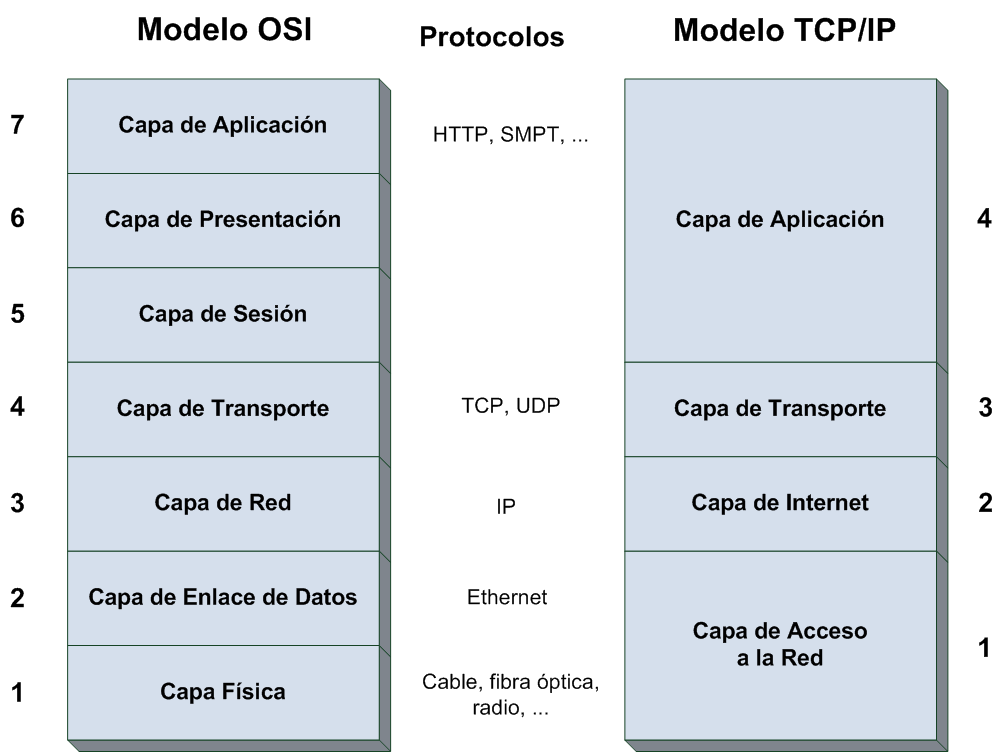
\includegraphics[width=1\textwidth]{imagenes/capas.png}
  \centering
  \caption{Modelos de capas de Internet.}
\end{figure}

\noindent Nosotros seguiremos el \textit{modelo TCP/IP}, y a continuación, procederemos a dar 
unas pinceladas sobre la capa de aplicación, la de transporte y la de enlace.

\subsection{Capa de aplicación}

En la capa de aplicación encontramos las aplicaciones de red y sus protocolos. 
Los protocolos que encontramos en esta capa son \textbf{HTTP, SMTP y FTP}. 
\intro
\begin{itemize}
\item El protocolo \textit{HTTP} permite la solicitud y transferencia de documentos web.
\item El protocolo \textit{SMTP} permite la transferencia de mensajes de correo electrónico.
\item El protocolo \textit{FTP} permite la transferencia de archivos entre dos terminales.
\end{itemize}

\noindent A parte de estos protocolos también corresponde a esta capa el \textbf{DNS}, 
que es el encargado de traducir los nombres de los sitios web.

\subsection{Capa de transporte}

La capa de transporte es la encargada de transportar los mensajes de la capa de aplicación. 
Los protocolos de esta capa son \textbf{TCP y UDP}. La principal diferencia y será algo que 
marque el trabajo es que \textit{TCP} está orientado a garantizar la conexión, mientras que \textit{UDP} no 
garantiza la conexión.

\subsection{Capa de red}

En la capa de red es donde nos encontramos el protocolo \textbf{IP} y también 
un protocolo, \textbf{ICMP}, que nuestro \textit{NMS} hay veces que localiza y 
sitúa junto con \textit{TCP y UDP}, aunque no pertenezca a la capa de transporte.
\intro
En esencia, esta capa es la que se encarga de transportar los \textit{datagramas} 
de un \textit{host} a otro.

\subsection{¿Qué es útil para nosotros?}

En nuestro caso nos quedaremos solamente en la capa de transporte, 
ignorando la información que podamos obtener de la capa 
de aplicación. En caso de que nuestro NMS lo detecte, incluiremos ICMP, 
pero solo para añadir más 
información a los distintos flujos que podemos llegar a analizar, 
pero despreciaremos la información relativa al resto de esta capa. 
El archivo pcap que utilizaremos para la prueba será \textit{nitroba.pcap}, 
el cual se puede obtener desde la web de Bro y el cual se corresponde con 
la obtención del tráfico de una universidad de Sudáfrica.
